\documentclass[11pt,a4paper,ngerman]{article}
\usepackage[bottom=2.5cm,top=2.5cm]{geometry} 
\usepackage{babel}
\usepackage[utf8]{inputenc} 
\usepackage[T1]{fontenc} 
\usepackage{ae} 
\usepackage{amssymb} 
\usepackage{amsmath}
\usepackage{amsthm} 
\usepackage{graphicx}
\usepackage{fancyhdr}
\usepackage{fancyref}
\usepackage{listings}
\usepackage{xcolor}
\usepackage{paralist}
\usepackage{tabularx}
\usepackage{tikz}
\usetikzlibrary{arrows,automata}
\usepackage[pdftex, bookmarks=false, pdfstartview={FitH}, linkbordercolor=white]{hyperref}
\usepackage{fancyhdr}
\pagestyle{fancy}
\fancyhead[C]{Diskrete Mathematik}
\fancyhead[L]{Übung 2}
\fancyhead[R]{SoSe 2013}
\fancyfoot{}
\fancyfoot[L]{}
\fancyfoot[C]{\thepage \hspace{1px} of \pageref{LastPage}}
\renewcommand{\footrulewidth}{0.5pt}
\renewcommand{\headrulewidth}{0.5pt}
\setlength{\parindent}{0pt} 
\setlength{\headheight}{0pt}

\date{}
\title{Übung 2}
\author{Max Wisniewski, Alexander Steen}


%%
%% Enviroments for proofs and lemmas
%%
\newtheorem{lemma}{\bfseries Claim}

\begin{document}

\lstset{language=Pascal, basicstyle=\ttfamily\fontsize{10pt}{10pt}\selectfont\upshape, commentstyle=\rmfamily\slshape, keywordstyle=\rmfamily\bfseries, breaklines=true, frame=single, xleftmargin=3mm, xrightmargin=3mm, tabsize=2, mathescape=true}

\renewcommand{\figurename}{Figure}

\maketitle
\thispagestyle{fancy}

\subsection*{Aufgabe 1.}
Sei $G = (V,E)$ ein Graph und $v \in V$ ein Blatt. \\
Zu zeigen: $G$ ist ein Baum $\Leftrightarrow$ $G' := (V \setminus \{v \}, E \setminus \delta(v))$ ist ein Baum. \\
\textbf{Beweis}:\\
"$\Rightarrow$": Sei $G$ ein Baum.\\
(1) In $G'$ kann kein Kreis entstanden sein, da keine Kanten hinzu kamen.\\
(2) $G'$ ist zusammenhängend: Da $v$ ein Blatt ist, gibt es genau einen Knoten, der adjazent zu $v$ ist.
Damit kann durch das Entfernen von $v$ keine neue Zusammenhangskomponente entstehen. 
\\
"$\Leftarrow$": Sei $G' := (V \setminus \{v \}, E \setminus \delta(v))$ ein Baum. \\
(1) $G$ ist kreisfrei: $G'$ war kreisfrei; der hinzugefügte Knoten $v$ kann nicht Teil eines
neuen Kreises sein da $d(v)=1$ gilt, jeder auf einem Kreis liegende Knoten aber mindestens Grad 2 haben muss.\\
(2) $G$ ist zusammenhängend,da keine Kanten entfernt worden sind und ein Knoten mit genau einer Kante hinzugefügt worden ist.
\mbox{}\hfill$\square$

\subsection*{Aufgabe 2.}
Zu zeigen: Ein Baum $G$ mit Maximalgrad $\Delta(G)$ hat mindestens $\Delta(G)$ Blätter.\\
Die Aussage ist offensichtlich falsch für Bäume mit unendlich vielen Knoten (man betrachte z.B.
einen unendlichen Pfad). Darum beschränken wir uns auf eine endliche Anzahl von Knoten.

\textbf{Beweis}:\\
Sei $G=(V,E)$ ein Baum mit $|V| < \aleph_0$ und Maximalgrad $\Delta(G)$.
D.h. es existiert ein Knoten $v \in V$ mit $d(v) = \Delta(G) =: d$. 
Falls $\Delta(G) = 0$
folgt die Behauptung direkt, also nehmen wir im folgenden $\Delta(G) \geq 1$ an.
Seien $G_1,\ldots,G_d$ die Unterbäume von $v$; dann gilt $1\leq |G_i| < \omega$. 
Seien $\tilde{G}_i$ die Bäume die man durch Hinzufügen von
(1) $v$ und (2) der Originalkante von $v$ nach $G_i$ aus $G_i$ enthält.
Nach dem ''Blattlemma'' (2.5) haben alle $\tilde{G}_i$ jeweils mindestens $2$ Blätter.
Betrachten wir also wieder den Originalgraphen $G = \bigcup \tilde{G}_i$, kann jedes
$\tilde{G}_i$ höchstens ein Blatt verloren haben (nämlich $v$ falls es nicht selber ein Blatt in $G$ ist). 
Damit enthält $G$ mindestens $\Delta(G)$ Blätter (in jedem $G_i$ eines).
\mbox{}\hfill$\square$

\pagebreak

\subsection*{Aufgabe 3.}
\textbf{Lösung:}\\

Wir haben den Namen \textbf{MAXWISNIE} gewählt. Ins Alphabet modulo $9$ und um eins inkrementiert ergibt sich der Code
$527612616$. Für den Algorithmus führen wir eine Liste mit markierten Knoten (müssen noch eingefügt werden
und stehen nicht in der Liste) und den verbleibenden Code. (Wir waren uns bei der Aufgabenstellung im unklaren ob
wir nun die ersten 9 oder die ersten 7 nehmen sollen)
\begin{table}[h!]
\centering
\begin{tabularx}{0.6\textwidth}{c|ccc}
Runde & Code & Marked & New Edge\\
\hline
0 & $527612616$ &  $\{3, 4, 8, 9, 10, 11\}$ & 5-3\\
1 & $27612616$ & $\{ 4, 5, 8, 9, 10, 11\}$ & 2-4\\
2 & $7612616$ & $\{ 5, 8, 9, 10, 11\}$ & 7-5\\
3 & $612616$ & $\{ 7, 8, 9, 10, 11\}$ & 6-7\\
4 & $12616$ & $\{ 8, 9, 10, 11\}$ & 1-8\\
5 & $2616$ & $\{ 9, 10, 11\}$ & 2-9\\
6 & $616$ & $\{ 2, 10, 11\}$ & 6-2\\
7 & $16$ & $\{ 10, 11\}$ & 1-10\\
8 & $6$ & $\{ 1, 11\}$ &6-1\\
9 & - & $\{ 6, 11\}$ & 6-11
\end{tabularx}
\caption{Ausführung der Decodierung vom Prüfercode}
\end{table}

Der dazugehörige Graph sieht wie folgt aus:

\begin{table}[h!]
\centering
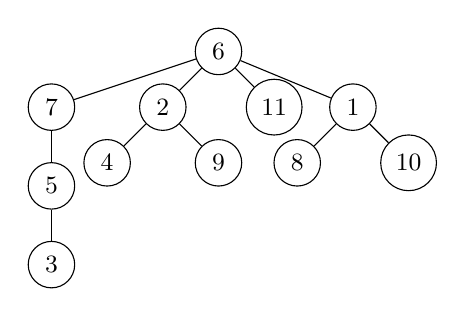
\begin{tikzpicture}[font=\small,minimum size=0.5cm]
	\node[circle,draw=black,name=6]{6};
	\node[circle,draw=black,name=11, below right of=6]{11};
	\node[circle,draw=black,name=2, below left of=6]{2};
	\node[circle,draw=black,name=4, below left of=2]{4};
	\node[circle,draw=black,name=1, right of=11]{1};
	\node[circle,draw=black,name=7, above left of=4]{7};
	\node[circle,draw=black,name=5, below of=7]{5};
	\node[circle,draw=black,name=3, below of=5]{3};
	\node[circle,draw=black,name=8, below left of=1]{8};
	\node[circle,draw=black,name=9, below right of=2]{9};
	\node[circle,draw=black,name=10, below right of =1]{10};

	\path[-] (3) edge (5)
		(5) edge (7)
		(7) edge (6)
		(11) edge (6)
		(9) edge (2)
		(4) edge (2)
		(2) edge (6)
		(10) edge (1)
		(8) edge (1)
		(1) edge (6);
\end{tikzpicture}
\caption{Baum für den Prüfercode $527612616$}
\end{table}


\subsection*{Aufgabe 4.}
\subsubsection*{a)}
Wie viele Klassen isomorpher Bäume gibt es in $T_5$? \\
\textbf{Lösung:}\\
Es gibt genau drei Klassen isomorpher Bäume:\\

\begin{tikzpicture}[font=\small,minimum size=0.5cm]
    \node[circle,draw=black,name=1] {};
    \node[circle,draw=black,name=2, right of=1] {};
    \node[circle,draw=black,name=3, left of=1] {};
    \node[circle,draw=black,name=4, above of=1] {};
    \node[circle,draw=black,name=5, below of=1] {};

    \node[circle,draw=black,name=6, right of=2, node distance=2cm] {};
    \node[circle,draw=black,name=7, right of=6] {};
    \node[circle,draw=black,name=8, right of=7] {};
    \node[circle,draw=black,name=9, above right of=8] {};
    \node[circle,draw=black,name=10, below right of=8] {};

    \node[circle,draw=black,name=11, right of=8, node distance=3cm] {};
    \node[circle,draw=black,name=12, right of=11] {};
    \node[circle,draw=black,name=13, right of=12] {};
    \node[circle,draw=black,name=14, right of=13] {};
    \node[circle,draw=black,name=15, right of=14] {};

    \path[-] (1) edge (2)
             (1) edge (3)
             (1) edge (4)
             (1) edge (5)
             (6) edge (7)
             (7) edge (8)
             (8) edge (9)
             (8) edge (10)
             (11) edge (12)
             (12) edge (13)
             (13) edge (14)
             (14) edge (15);
\end{tikzpicture}

(1) Alle isomorphen Bäume mit maximaler Pfadlänge 3 (links).\\
(2) Alle isomorphen Bäume mit maximaler Pfadlänge 4 (mitte).\\
(3) Alle isomorphen Bäume mit maximaler Pfadlänge 5 (rechts).
\subsubsection*{b)}
Gesucht: $|[T]|$ für alle Isomorphieklassen.
Seien $T_1, T_2, T_3$ die Bäume aus (a), dann ist:
\begin{enumerate}
\item $|[T_1]| = 5$
\item $|[T_2]| = 120$
\item $|[T_3]| = 120$ 
\end{enumerate}
$T_2, T_3$ ergeben sich, da wenn man einmal spiegelt wieder der selbe Graph herraus kommt. Daher haben wir $5! / 2$ viele
Isomorphismen. Bei $T_1$ können wir wählen welches der 5 Elemente wir in die Mitte stellen. Danach sind alle Graphen gleich.
\subsubsection*{c)}

$\sum_{[T]} |[T]| = |[T_1]| + |[T_2]| + |[T_3]| = 5 + 60 + 60 = 125 = 5^3$
Dieses Ergebnis ist auch sinvoll, da die Summe alle Bäume ergeben muss und wir nach dem Satz von Caley
wissen, dass dies eben $125$ sind. 

\label{LastPage}

\end{document}
